\documentclass[aspectratio=169]{beamer}

\usepackage{style}

\begin{document}
\onehalfspacing

%---------------------------------------------------------

% Oznaczenia języków
\newcommand{\D}{\mathcal{D}}
\newcommand{\E}{\mathcal{E}}
\newcommand{\C}{\mathcal{C}}

%---------------------------------------------------------

\frame{\titlepage}

%---------------------------------------------------------

% \begin{frame}{Notatki}
%     \begin{enumerate}
%         \item homomorfizm grafów
%         \item \(k\)-kolorowanie \( \rightarrow \) klika
%         \item homomorfizmy konkretnego grafu (?)
%         \item 2-kolorowanie \( \rightarrow \) krawędź
%         \item Tw: nieskierowany i niedwudzielny, to NP
%         \item czyli umiemy scharakteryzować grafy, które są łatwe
%         \item Hipoteza: dychotomia dla grafów bez źródeł i ujść
%         \item pp-metody: definicje (małe zmiany), interpretacje (homomorficzne równoważności), konstrukcje (stałe)
%         \item Chcemy definiować, żeby mieć lepszą kontrolę i móc przenieść na nieskończoność
%     \end{enumerate}
% \end{frame}

%---------------------------------------------------------

\begin{frame}{Graph homomorphism}

\begin{columns}
\column{0.5\textwidth}
\textcolor{cfred}{Homomorphism} \\
Given graphs \(G\) and \(H\), a mapping \\
\hspace{1.5cm} \( f : V (G) \to V (H) \) \\
is a homomorphism from \(G\) to \(H\) iff
\((u, v) \in E(G) \Longrightarrow \big(f (u), f (v)\big) \in E(H)\)

\vspace{1.5em}
\only<2>{
\textcolor{cfred}{Core} \\
Graph $H$ is a core if every endomorphism of $H$ is a bijection.
}

\column{0.5\textwidth}
\begin{figure}
    \centering
    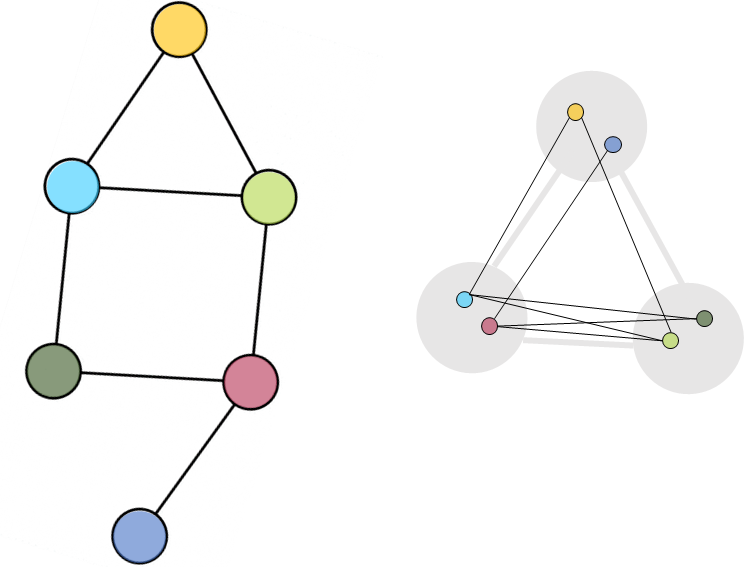
\includegraphics[width=0.95\linewidth]{images/hom.png}
\end{figure}
\end{columns}

\end{frame}

%---------------------------------------------------------

\begin{frame}{\(H\)-colouring}


\begin{columns}
\column{0.01\textwidth}
\column{0.5\textwidth}
\textcolor{cfred}{\(H\)-colouring} \\
A graph \(G\) is \(H\)-colourable iff there exists a homomorphism to a fixed graph \(H\). \\

\vspace{1.5em}
\only<2>{A graph \(G\) is \(n\)-colourable iff there exists a homomorphism \( G \to K_n\).}

\column{0.5\textwidth}
\begin{figure}
    \centering
    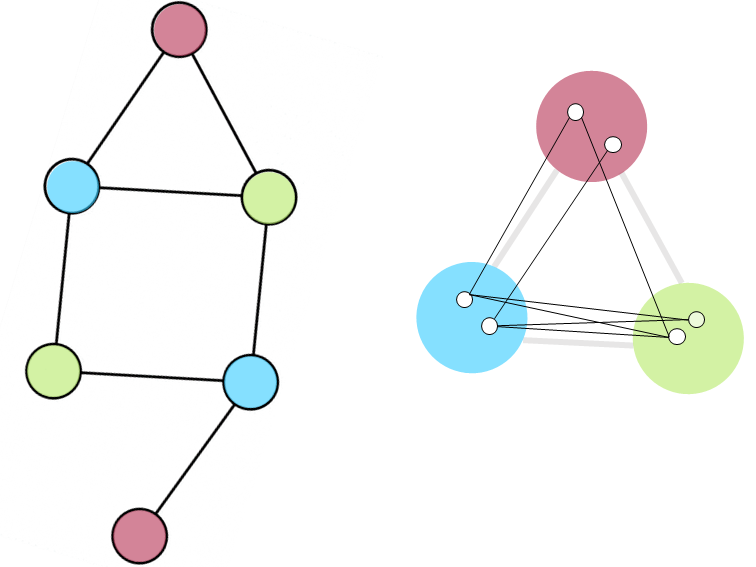
\includegraphics[width=0.75\linewidth]{images/col1.png}
\end{figure}
\end{columns}

\end{frame}

%---------------------------------------------------------

\begin{frame}{Dichotomy}

\textcolor{cfblue}{Hell-Nešetřil dichotomy} \\
If \( H \) is bipartite, or contains a loop, then \(H\)-colouring is in P, otherwise is NP-hard.

\pause
\vspace{1.5em}
For a fixed graph \(H\), deciding whether a give graph is \(H\)-colourable is either NP-complete or solvable in polynomial time.

\end{frame}

%---------------------------------------------------------

\begin{frame}{CSP}

An instance of the CSP is
\begin{itemize}
    \item \(V\) a finite set of variables,
    \item \(D\) a finite domain,
    \item \(\C\) a finite list of constraints
\end{itemize}

\end{frame}

%---------------------------------------------------------

\begin{frame}{SAT as CSP(\(\C\))}

\[ \C = \set{R_{ijk} : i, j, k \in \set{0, 1}}, \text{ where } R_{ijk} = \set{0, 1}^3 \setminus \set{(i, j, k)} \]

\pause
\vspace{1.5em}
\[ \varphi = (x_1 \lor \neg x_2 \lor x_3) \land (\neg x_4 \lor x_5 \lor \neg x_1) \]
\[ \C_{\varphi} = \set{R_{010}(x_1, x_2, x_3), R_{101}(x_4, x_5, x_1)} \]


\end{frame}

%---------------------------------------------------------

\begin{frame}{Pp-definition}

Let \( \D, \E \) be constraint languages on the same domain \( D = E \). \\

\vspace{0.5em}
Language \(\D\) pp-defines \(\E\) if each relation in \(\E\) can be defined by a first order formula which only uses relations in \(\D\), \(=\), \(\land\) and \(\exists\).

\pause
\vspace{2em}
If \(\D\) pp-defines \(\E\), then \(CSP(\E)\) is reducible to \(CSP(\D)\).

\end{frame}

% ---------------------------------------------------------

\begin{frame}{Pp-definition -- example}
Negation in 1-in-3-SAT can be defined as 
\[
    \neg x = \exists_{a,b} \ R(x,a,b) \land R(a,b,b)
\]
% a albo b muszą być prawdziwe, więc jeśli x prawdziwe to formuła fałszywa i odwrotnie
\pause
\vspace{1.5em}
To pp-define 3-SAT with 1-in-3-SAT it suffices to write
\vspace{-1em}
\[
    (x \lor y \lor z) = \exists_{a,b,c,d} \ R(\neg x, a, b) \land R(b, y, c) \land R(c, d, \neg z) 
\]

\end{frame}

% ---------------------------------------------------------

\begin{frame}{no Pp-definition -- example}
% A relation \(\E\) is not pp definable in \(\D\) if  \(\D\) is not preserved by all homomorphisms of \(\E\).

It is not possible to pp-define 3-SAT with NAE-3-SAT, as NAE-3-SAT is symmetric.\\
\pause
\vspace{1em}
More formally NAE-3-SAT is closed under \(f(x)=\neg x\), while 3-SAT is not. Therefore 3-SAT cannot be pp-defined in NAE-3-SAT.

\end{frame}

% ---------------------------------------------------------

% \begin{frame}{pp-interpretation}

% Let \( \D, \E \) be constraint languages. \\

% \vspace{0.5em}
% Language \(\D\) pp-interprets \(\E\) if there exist \(n \in \mathbb{N}\), a set \( F \subseteq D^n \), and a mapping \( f : F \rightarrow E \) such that \(\D\) pp-defines
% \begin{itemize}
%     \item the relation \(F\),
%     \item \(f^{-1}(=_E)\),
%     \item \(f^{-1}(R)\) for every relation \(R\) in \(\E\),
% \end{itemize}
% where \(f^{-1}(R)\) for \(R \subseteq E^k\) is the \(nk\)-ary relation on \(D\) defined by \\
% \( f^{-1}(R)(x_{11}, \ldots, x_{1k}, x_{21}, \ldots, x_{2k}, \ldots, x_{n1}, \ldots, x_{nk}) \) \\
% \hspace{5cm}\( \iff R(f(x_{11}, \ldots, x_{n1}), \ldots, f(x_{1k}, \ldots, x_{nk})) \).

% \end{frame}

%---------------------------------------------------------

% \begin{frame}{pp-construction}

% Let \( \D, \E \) be constraint languages. \\

% \vspace{0.5em}

% Language \(\D\) pp-constructs \(\E\) if there is a sequence of constraint languages
% \[ \D = \C_1,...,\C_k = \E \]
% such that, for each \(1 \leq i < k\)
% \begin{itemize}
%     \item \(\C_i\) pp-interprets \(\C_{i+1}\),
%     \item or \(\C_i\) is homomorphically equivalent to \(\C_{i+1}\),
%     \item or \(\C_i\) is a core and \(\C_{i+1}\) is \(C_i\) extended with constants.
% \end{itemize}

% \end{frame}

%---------------------------------------------------------

% \begin{frame}{pp-methods}
% \begin{figure}[!ht]
% \centering
% \resizebox{1\textwidth}{!}{%
% \begin{circuitikz}[every node/.style={font=\normalsize}]
%     % Nodes
%     \node [font=\LARGE] (def) at (1.5,15.75) {pp-definition};
%     \node [font=\LARGE] (interp) at (6.75,15.75) {pp-interpretation};
%     \node [font=\LARGE] (cons) at (12.5,15.75) {pp-construction};
    
%     \node [font=\LARGE] at (3.75,15.75) {$\subseteq$};
%     \node [font=\LARGE] at (9.75,15.75) {$\subseteq$};
    
%     \draw [->, >=Stealth, draw=cfred] (1.25,15.25) .. controls (2.75,14) and (4,14) .. (5.75,15.25) 
%         node[midway, below, font=\normalsize] {+ change of domain};
    
%     \draw [->, >=Stealth, draw=cfred] (7.75,15.2) .. controls (9.25,14) and (10.5,14) .. (12.25,15.25) 
%         node[midway, below, font=\normalsize] {+ adding constants in cores};
% \end{circuitikz}
% }%
% \end{figure}

% \pause
% \vspace{1em}
% If \(\D\) pp-constructs \(\E\), then \(CSP(\E)\) is reducible to \(CSP(\D)\).

% \end{frame}

%---------------------------------------------------------

\begin{frame}{Dichotomy}

\textcolor{cfblue}{CSP Dichotomy} \\
For a relational structure \(T\) the problem CSP\((T)\) is either NP-complete \\
or solvable in polynomial time.

\pause
\vspace{1.5em}
\textcolor{cfblue}{Conjecture (Bang-Jensen and Hell)} \\
Let \(H\) be a graph without sources or sinks. If each component of the core of \(H\) is~a~cycle, then \(CSP(H)\) is polynomially decidable. Otherwise \(CSP(H)\) is NP-complete.

\end{frame}

%---------------------------------------------------------

\begin{frame}{Sources}

\begin{itemize}
    \item Libor Barto, Andrei Krokhin, Ross Willard,\\
    \href{https://drops.dagstuhl.de/storage/02dagstuhl-follow-ups/dfu-vol007/DFU.Vol7.15301.1/DFU.Vol7.15301.1.pdf}{\textit{Polymorphisms, and How to Use Them}}, 2017.
    \item Libor Barto, Marcin Kozik, Todd Ninven,\\
    \href{https://www.karlin.mff.cuni.cz/~barto/Articles/CSPSmooth.pdf}{\textit{The CSP Dichotomy Holds For graphs With No Sources And No Sinks}}, 2009.
    \item Sebastian Meyer, Jakub Opr\v sal, \href{https://arxiv.org/abs/2409.12627}{\textit{A topological proof of the Hell-Ne\v set\v ril dichotomy}}, 2024.
\end{itemize}

\end{frame}

%---------------------------------------------------------


\end{document}